  \documentclass[12pt]{article}
\usepackage[pdftex]{graphicx}
\usepackage{amsmath}
\usepackage{bibentry}
\usepackage{ccaption}
\usepackage{fourier}
\usepackage{stata}
\usepackage[margin= 1in]{geometry}

\usepackage[colorlinks=true,
                      pdfstartview=FitV,
                      urlcolor=blue,
]{hyperref}

\usepackage{natbib}

\begin{document}

\thispagestyle{empty}%

\setlength{\parskip}{1ex plus 0.5ex minus 0.2ex}

\setcounter{secnumdepth}{-2}


\begin{flushleft}
Vanderbilt University\\Leadership, Policy and Organizations\\Class Number 9522\\ Spring 2018
\end{flushleft}

\begin{center}
\textbf{Working With Panel Data}
\end{center}

\section{Introduction}

Panel data refers to data with multiple observations per unit. In
education settings panel data is almost more common than not, with
many studies involving cases that have been observed over time.

For all of the models below, I'll use the following notation:

$y_{it}$ is the dependent variable for unit $i$ ($i=1 \ldots n$) in time period $t$ ($t= 1 \ldots t$). 

$x_{it}$ is an independent variable for unit $i$ at time $t$. 

$\beta$ is a coefficient on the variable $x$

$\epsilon_{it}$ is an error term


The terminology around panel data can be confusing, because economists
and education experts discuss the same things using different
names. Here's some terminology:

\begin{description}
\item \emph{Panel data}: when used by economists, this typically
  refers to a dataset where there are many more units than
  observations over time. 

\item \emph{Cross-sectional time-series data}: this refers to data
  where there are much longer time series, and fewer data points. 

\item \emph{Hierarchical or ``grouped'' data}: this refers to data
  where the observations are naturally grouped, e.g. students in
  classrooms, classrooms in schools. This type of data can also
  include multiple observations over time. 

\item \emph{Fixed effects}:when used by economists, this refers to
  models where the group mean is controlled for, either by subtracting
  it from the dependent variable or by individually controlling for
  each group effect via dummy variables. Also known as LSDV: least
  squares dummy variables. When HLM people say fixed effects, they're
  referring to coefficients that don't vary across groups. This is
  also known as a ``no pooling'' model. 


\item \emph{Random effects}: when used by economists, this refers to a
  model that allows one or more coefficients to have its own
  distribution with an error term. A random effects model is
  functionally equivalent to a Hierarchical Linear Model, although HLM
  imposes additional assumptions. 


\end{description}

\section{Describing Panel Data}

The data we'll be using come from my dissertation, which prediction
appropriations, tuition and financial aid at the state level using
various characteristics of the political and higher education
system. The data are a balanced panel of 49 states (excluding Alaska)
over 16 years, 1984-1999. 

To get Stata to recognize this as panel data, we need to use the xtset
command. 

\begin{stlog}
  . /* Set up data as panel data */
. xtset state year, yearly
       panel variable:  state (strongly balanced)
        time variable:  year, 1984 to 1999
                delta:  1 year
\end{stlog}

I tend to use two basic methods for describing panel data. First, I
like to do line graphs for all of the continuous variables, which give
you a very clear sense of variation across units and any time
trends. It's also a good way to find data problems:

\begin{stlog}
. xtline approps_i  
\end{stlog}



\begin{figure}[h]
  \centering
  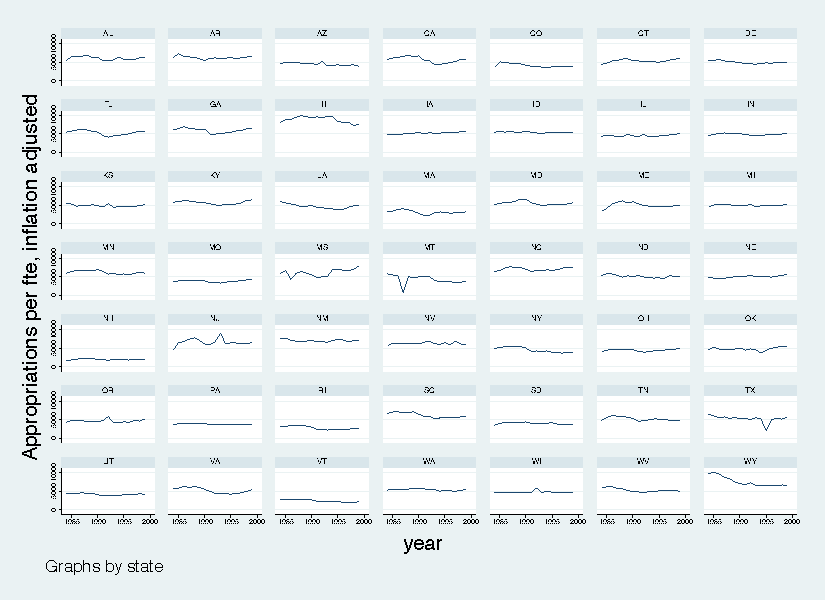
\includegraphics[width=\textwidth]{app_line}
  \caption{Trend in Appropriations Per Student, by State}
\end{figure}

\begin{stlog}
. xtline pub4tuit_i
\end{stlog}

\begin{figure}[h]
  \centering
  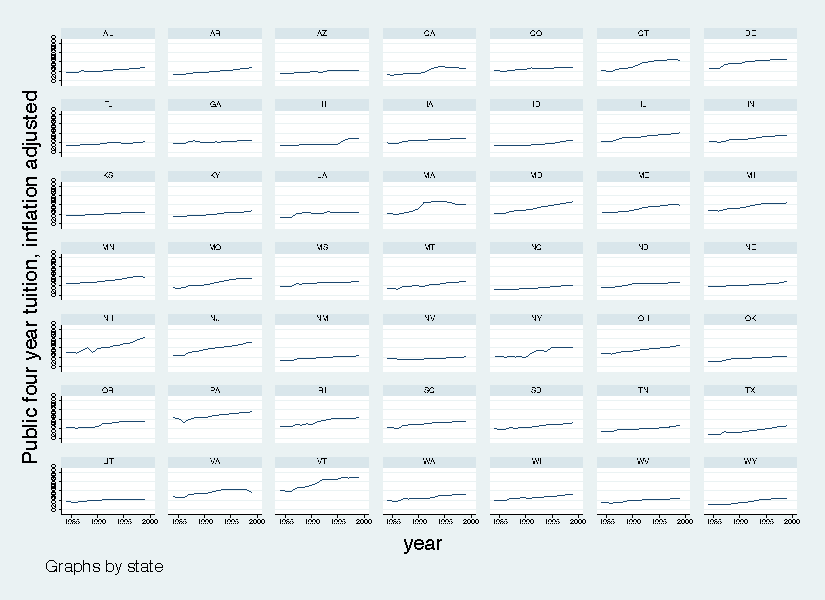
\includegraphics[width=\textwidth]{tuit_line}
  \caption{Trend in Public Four-Year Tuition, by State}
\end{figure}


The other graph I like to use is a boxplot for the variable by
state. This gives an excellent sense of variability both across and
within units. 

\begin{stlog}
. 
. #delimit ;
delimiter now ;
. graph hbox pub4tuit_i,
> over(state, sort(1) descending label(labsize(tiny) )) 
> 
> ;  
\end{stlog}


\begin{figure}[h]
  \centering
  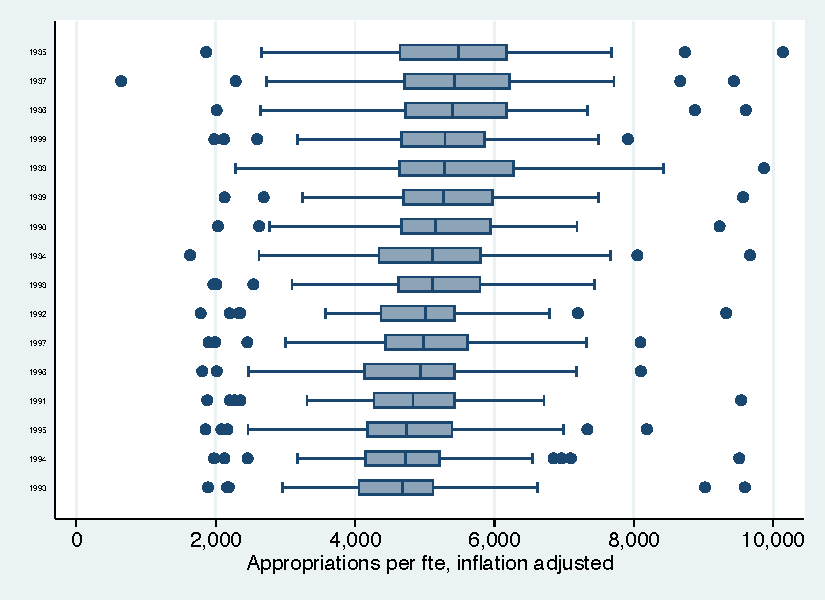
\includegraphics[width=\textwidth]{approps_box}
  \caption{Variation in Appropriations Per Student, by State}
\end{figure}


\begin{stlog}
  . #delimit ;
delimiter now ;
. graph hbox approps,
> over(state, sort(1) descending label(labsize(tiny) )) 
> ;
\end{stlog}


\begin{figure}[h]
  \centering
  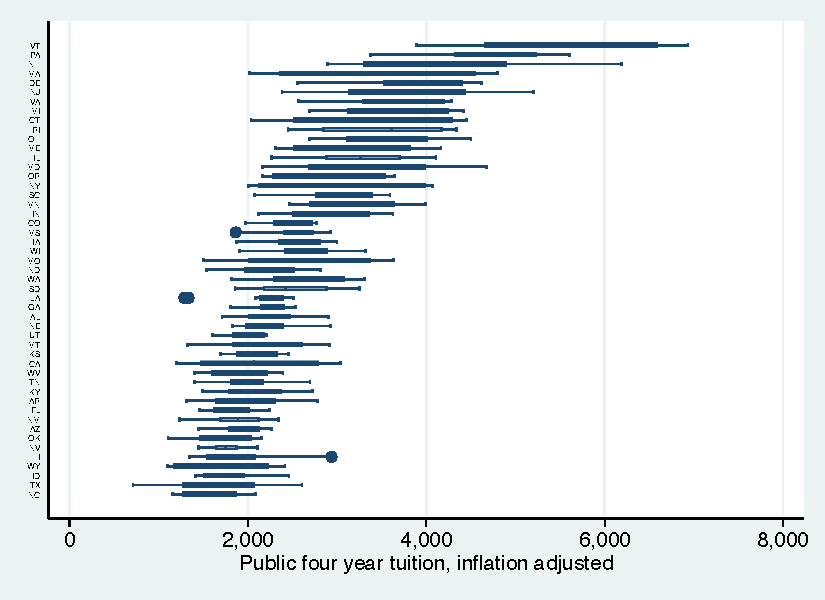
\includegraphics[width=\textwidth]{tuit_box}
  \caption{Variation in Public Four-Year Tuition, by State}
\end{figure}


When reporting descriptives for a panel dataset, don't just give the
grand mean. Provide averages and standard deviations for a subset of
time periods, along with graphics similar to the above. 

\section{Ordinary Least Squares}

The OLS estimate for panel data is: 

\begin{equation*}
  \label{eq:ols}
  y_{it}=\alpha+ \beta x_{it} + \epsilon_{it}
\end{equation*}


In Stata:

\begin{stlog}
  . 
. local y approps_i

. 
. local controls perc1824 incpcp_i percpriv taxcpc_i  legcomp_i i.board 

. 
. reg `y'  legideo `controls'

      Source |       SS       df       MS              Number of obs =     784
-------------+------------------------------           F( 10,   773) =  111.00
       Model |   830964034    10  83096403.4           Prob > F      =  0.0000
    Residual |   578657976   773   748587.29           R-squared     =  0.5895
-------------+------------------------------           Adj R-squared =  0.5842
       Total |  1.4096e+09   783  1800283.54           Root MSE      =  865.21

------------------------------------------------------------------------------
   approps_i |      Coef.   Std. Err.      t    P>|t|     [95% Conf. Interval]
-------------+----------------------------------------------------------------
     legideo |   1.954075   1.373991     1.42   0.155    -.7431209    4.651272
    perc1824 |   267.1039   29.04555     9.20   0.000     210.0865    324.1214
    incpcp_i |  -12.65837   12.94071    -0.98   0.328    -38.06147    12.74473
    percpriv |  -57.78148   2.810894   -20.56   0.000    -63.29937   -52.26359
    taxcpc_i |   1.939732   .1145756    16.93   0.000     1.714816    2.164649
   legcomp_i |  -.0008065   .0020159    -0.40   0.689    -.0047638    .0031508
             |
       board |
          2  |   110.3047   100.8765     1.09   0.275    -87.71972    308.3291
          3  |  -28.19471   94.82565    -0.30   0.766     -214.341    157.9516
          4  |   -29.0085   87.02584    -0.33   0.739    -199.8435    141.8265
          5  |  -1538.795   143.7325   -10.71   0.000    -1820.947   -1256.643
             |
       _cons |   944.5651   466.3937     2.03   0.043     29.01674    1860.113
------------------------------------------------------------------------------

. 
\end{stlog}


The problem with the OLS model is both that it may be inconsistent and
that it may induce huge problems with heteroscedasticity. If you're
not sure if you there's a problem, try graphing the residuals like so: 


\begin{stlog}
  . predict e, resid

. 
. graph box e, over(state, sort(1) descending label(labsize(tiny))) /*Horrible*/

\end{stlog}


\begin{figure}[h]
  \centering
  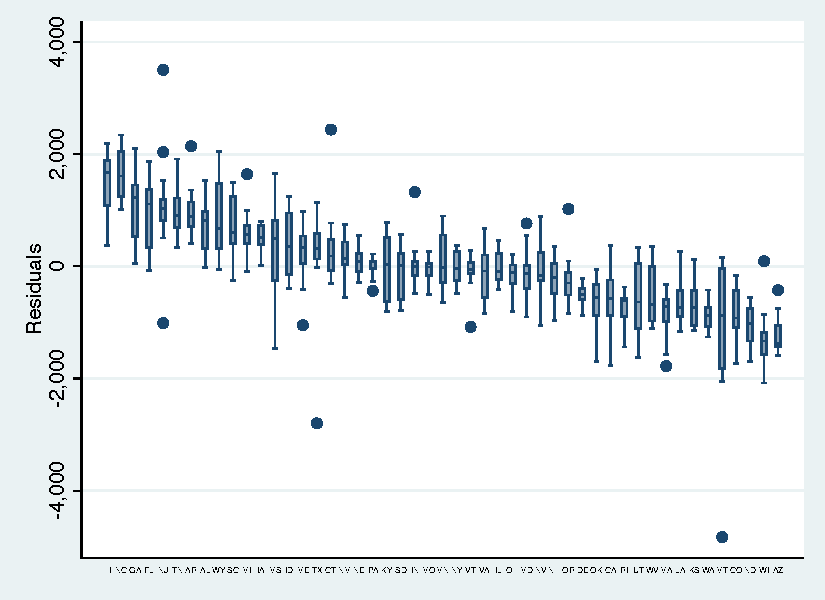
\includegraphics[width=\textwidth]{resid_state}
  \caption{Residuals by State}
\end{figure}


\begin{figure}[h]
  \centering
  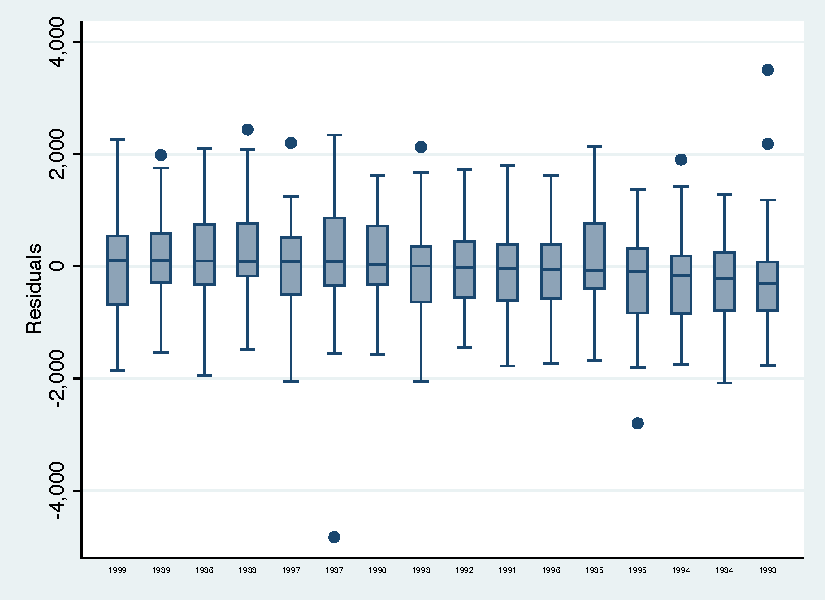
\includegraphics[width=\textwidth]{resid_year}
  \caption{Residuals by Year}
\end{figure}

In our case, there are massive problems with the error terms by
state. It's not so bad by year. Even so, we will have a correlation
with the independent variables and the error term becuase we're
leacving out a variable that is known to impact the dependent
variable: the group that each unit is in. 

\section{Fixed Effects Models}


The fixed effects model with group specific intercepts is: 

\begin{equation*}
  \label{eq:ols}
  y_{it}=\alpha_i+ \beta x_{it} + \epsilon_{it}
\end{equation*}


A basic fixed effects model looking at the effect of a more liberal
government on appropriations would be specified as:


\begin{stlog}
. xi: xtreg `y'  legideo `controls', fe
i.board           _Iboard_1-5         (naturally coded; _Iboard_1 omitted)
note: _Iboard_5 omitted because of collinearity

Fixed-effects (within) regression               Number of obs      =       784
Group variable: state                           Number of groups   =        49

R-sq:  within  = 0.2281                         Obs per group: min =        16
       between = 0.0860                                        avg =      16.0
       overall = 0.1015                                        max =        16

                                                F(9,726)           =     23.83
corr(u_i, Xb)  = -0.2562                        Prob > F           =    0.0000

------------------------------------------------------------------------------
   approps_i |      Coef.   Std. Err.      t    P>|t|     [95% Conf. Interval]
-------------+----------------------------------------------------------------
     legideo |   3.508206   1.188178     2.95   0.003     1.175531    5.840881
    perc1824 |   269.2799   24.15645    11.15   0.000     221.8551    316.7048
    incpcp_i |   12.85631   20.06298     0.64   0.522    -26.53207    52.24468
    percpriv |  -3.949699   10.39503    -0.38   0.704    -24.35761    16.45821
    taxcpc_i |   1.436178   .1566408     9.17   0.000     1.128655    1.743701
   legcomp_i |   .0022197    .001997     1.11   0.267    -.0017009    .0061402
   _Iboard_2 |  -41.50431   108.1897    -0.38   0.701    -253.9063    170.8977
   _Iboard_3 |  -597.6449   204.1981    -2.93   0.004    -998.5342   -196.7557
   _Iboard_4 |  -942.1278   183.3558    -5.14   0.000    -1302.099   -582.1569
   _Iboard_5 |  (omitted)
       _cons |  -38.59943   659.1182    -0.06   0.953    -1332.605    1255.406
-------------+----------------------------------------------------------------
     sigma_u |  1232.7514
     sigma_e |  492.51715
         rho |  .86235025   (fraction of variance due to u_i)
------------------------------------------------------------------------------
F test that all u_i=0:     F(48, 726) =    34.57             Prob > F
= 0.0000

. xi: reg `y' legideo `controls' i.state
i.board           _Iboard_1-5         (naturally coded; _Iboard_1 omitted)
i.state           _Istate_2-50        (naturally coded; _Istate_2 omitted)
note: _Istate_22 omitted because of collinearity

      Source |       SS       df       MS              Number of obs =     784
-------------+------------------------------           F( 57,   726) =   89.21
       Model |  1.2335e+09    57  21640594.9           Prob > F      =  0.0000
    Residual |   176108102   726  242573.144           R-squared     =  0.8751
-------------+------------------------------           Adj R-squared =  0.8653
       Total |  1.4096e+09   783  1800283.54           Root MSE      =  492.52

------------------------------------------------------------------------------
   approps_i |      Coef.   Std. Err.      t    P>|t|     [95% Conf. Interval]
-------------+----------------------------------------------------------------
     legideo |   3.508206   1.188178     2.95   0.003     1.175531    5.840881
    perc1824 |   269.2799   24.15645    11.15   0.000     221.8551    316.7048
    incpcp_i |   12.85631   20.06298     0.64   0.522    -26.53207    52.24468
    percpriv |  -3.949699   10.39503    -0.38   0.704    -24.35761    16.45821
    taxcpc_i |   1.436178   .1566408     9.17   0.000     1.128655    1.743701
   legcomp_i |   .0022197    .001997     1.11   0.267    -.0017009    .0061402
   _Iboard_2 |  -41.50431   108.1897    -0.38   0.701    -253.9063    170.8977
   _Iboard_3 |  -597.6449   204.1981    -2.93   0.004    -998.5342   -196.7557
   _Iboard_4 |  -942.1278   183.3558    -5.14   0.000    -1302.099   -582.1569
   _Iboard_5 |  -1876.622   218.9806    -8.57   0.000    -2306.533   -1446.711
   _Istate_3 |   276.3964   184.0882     1.50   0.134    -85.01223    637.8051
   _Istate_4 |  -933.8803   259.3431    -3.60   0.000    -1443.032
   -424.7282

....
  
\end{stlog}

This includes both the standard \texttt{xtreg} command and a
\texttt{reg} command, with xi specified to control for state level
effects. The coefficients are the same.  The interpretation of a fixed
effects model always refers only to within-unit changes in both the
independent and dependent variables. 

Without correcting for time in the above model, we could introduce
serially correlated error terms.

\section{Fixed Effects for Time}

In addition to specifying fixed effects for groups, the simplest
approach to handling time is to specify fixed effects for time, with
T-1 variables for time included in the model, with a new set of
coefficients $\gamma_t$. 

\begin{equation*}
  \label{eq:fe-time}
  y_{it}=\alpha_i+ \beta x_{it} + \gamma_t + \epsilon_{it}
\end{equation*}

To estimate the above in stata, we would need to use the \texttt{i}
function, which transforms variables into a categorical variable. The
following syntax gives fixed effects for time, with time as a
categorical variable:

\begin{stlog}
 
. 
. /* Fixed Effects for Units and Time (state and year) */
. 
.  xtreg `y' legideo  `controls'  i.year , fe
note: 5.board omitted because of collinearity

Fixed-effects (within) regression               Number of obs      =       784
Group variable: state                           Number of groups   =        49

R-sq:  within  = 0.3942                         Obs per group: min =        16
       between = 0.0321                                        avg =      16.0
       overall = 0.0576                                        max =        16

                                                F(24,711)          =     19.27
corr(u_i, Xb)  = -0.4822                        Prob > F           =    0.0000

------------------------------------------------------------------------------
   approps_i |      Coef.   Std. Err.      t    P>|t|     [95% Conf. Interval]
-------------+----------------------------------------------------------------
     legideo |   1.145978   1.140491     1.00   0.315    -1.093154    3.385111
    perc1824 |   44.91926   30.75181     1.46   0.145    -15.45595    105.2945
    incpcp_i |   139.2413   28.45662     4.89   0.000     83.37225    195.1104
    percpriv |  -3.777036   10.16795    -0.37   0.710    -23.73984    16.18577
    taxcpc_i |   1.501035   .1425019    10.53   0.000      1.22126     1.78081
   legcomp_i |   .0016732   .0018213     0.92   0.359    -.0019025     .005249
             |
       board |
     cbweak  |  -24.88159   97.00964    -0.26   0.798    -215.3412     165.578
      gball  |  -454.4452   183.9582    -2.47   0.014    -815.6115   -93.27897
     gbfour  |  -711.7997   165.6897    -4.30   0.000    -1037.099   -386.5002
       plan  |          0  (omitted)
             |
        year |
       1985  |   220.3299   90.99408     2.42   0.016     41.68063    398.9791
       1986  |   113.4229     97.881     1.16   0.247    -78.74752    305.5932
       1987  |  -19.38342   105.0826    -0.18   0.854    -225.6928     186.926
       1988  |  -67.57019   113.1309    -0.60   0.551    -289.6807    154.5403
       1989  |  -274.3213   122.1241    -2.25   0.025    -514.0883   -34.55431
       1990  |  -399.1526   125.7373    -3.17   0.002    -646.0135   -152.2917
       1991  |  -657.3481   125.0003    -5.26   0.000    -902.7619   -411.9343
       1992  |  -678.0808   134.1735    -5.05   0.000    -941.5044   -414.6571
       1993  |   -936.106   136.6561    -6.85   0.000    -1204.404   -667.8083
       1994  |  -968.5213   145.4102    -6.66   0.000    -1254.006   -683.0365
       1995  |  -1031.559   153.3461    -6.73   0.000    -1332.624   -730.4935
       1996  |  -1044.886   162.4511    -6.43   0.000    -1363.827   -725.9445
       1997  |  -1058.236   171.5086    -6.17   0.000     -1394.96   -721.5123
       1998  |  -1197.384   189.6214    -6.31   0.000    -1569.669   -825.0989
       1999  |  -1194.228   195.1562    -6.12   0.000    -1577.379   -811.0763
             |
       _cons |  -163.0829   776.2306    -0.21   0.834    -1687.061    1360.895
-------------+----------------------------------------------------------------
     sigma_u |   1421.003
     sigma_e |  440.90254
         rho |  .91218326   (fraction of variance due to u_i)
------------------------------------------------------------------------------
F test that all u_i=0: F(48, 711) = 52.77                    Prob > F = 0.0000

. 
\end{stlog}


The interpretation of this would be as usual for a categorical
variable: each coefficent for time represents a contrast to a base
time period (stata will choose the first one). Having done this
however, concerns about serial correlation should be adequately
addressed. 

 This can be observed by looking at a boxplot of errors by
 time period:

 \texttt{predict res,e}
 \texttt{graph box res, over(year)}


 \begin{figure}
   \centering
   \includegraphics[width=\textwidth]{box_year}
   \caption{Plot of Residuals by Year, Fixed Effects for Time}
   \label{fig:fetime}
 \end{figure}

Fixed effects for time are not symmetric with fixed effects for groups
in this model. To adjust for this, we can regress 

$y_{*it}= y_{it}-\bar{y}_{i}-\bar{y}_{t}+\bar{y}$

on the independent variable x, specified as: 

$x_{*it}= x_{it}-\bar{x}_{i}-\bar{x}_{t}+\bar{x}$


\section{Serially Correlated Errors}

Fixed effects for time is an appropriate approach in many cases,
however it is very inefficient: if time itself is not of interest, you
will have $T-1$ nuisance parameters along with $n-1$ group estimates
in the case of a fixed effects approach. 

When estimating models for panel data, corrections for autocorrelation
are much the same as in a single sample. First, assume that there is
no cross-sectional autocorrelation:

\begin{equation*}
  \label{eq:noauto}
  \text{Corr}[\epsilon_{it}.\epsilon_{js}]=0 \text{, if } i \neq j
\end{equation*}

In the presence of within-unit autocorrelation, the observed error $\epsilon_{it}$
consists of two parts: the error term in the previous year multiplied
by a coefficient $\rho$ and the overall error term $\mu_{it}$.

\begin{equation*}
  \label{eq:ar1}
  \epsilon_{it}=\rho_i \epsilon_{it-1}+\mu_{it}
\end{equation*}

The variance of these group-specific error terms is therefore:

\begin{equation*}
  \text{Var}[\epsilon_{it}]=\sigma^2_i=\frac{\sigma^2 _\mu i}{1-\rho^2_i}
\end{equation*}

To account for this, we need to calculate a correlation coefficient
$\rho$ for each group. A group specific estimate $r_i$ for $\rho$ is:

\begin{equation*}
  r_i=\frac{\sum_{t=2} ^{T} e_{it} e_{i,t-1}}{\sum_{t=1} ^{T}e^2_{it}}
\end{equation*}

Most programs, including STATA, calculate a single value, which is the
average of all group specific correlation coefficients. This value is
then used to transform the data to eliminate the autocorrelation. For
instance for $y_it$, the transformation is:

\begin{equation*}
  y_{i1}, y_{i2},\ldots y_{iT}= \sqrt{1-r^2}y_i1, y_{i2}-r_i y_{i1},
  y_{i3}-r_i y_{i2}, y_{iT}-r_iy_{i,T-1}
\end{equation*}


To estimate a fixed effects model in STATA, use the \texttt{xtregar}
command. In our running example, this can be estimated via: 

\begin{stlog}
  
. xi: xtregar `y' legideo `controls', fe rhotype (tsc) twostep lbi
i.board           _Iboard_1-5         (naturally coded; _Iboard_1 omitted)
note: _Iboard_5 dropped because of collinearity

FE (within) regression with AR(1) disturbances  Number of obs      =       735
Group variable: state                           Number of groups   =        49

R-sq:  within  = 0.1475                         Obs per group: min =        15
       between = 0.0584                                        avg =      15.0
       overall = 0.0235                                        max =        15

                                                F(9,677)           =     13.02
corr(u_i, Xb)  = -0.6379                        Prob > F           =    0.0000

------------------------------------------------------------------------------
   approps_i |      Coef.   Std. Err.      t    P>|t|     [95% Conf. Interval]
-------------+----------------------------------------------------------------
     legideo |   2.203477   1.328746     1.66   0.098    -.4054819    4.812437
    perc1824 |   308.6154   33.12758     9.32   0.000     243.5702    373.6605
    incpcp_i |   16.72646   23.96317     0.70   0.485    -30.32461    63.77753
    percpriv |   39.45439   12.99704     3.04   0.002     13.93505    64.97374
    taxcpc_i |   .9035681   .1776652     5.09   0.000     .5547272    1.252409
   legcomp_i |   .0015629   .0019213     0.81   0.416    -.0022095    .0053352
   _Iboard_2 |  -88.92507   136.4487    -0.65   0.515    -356.8385    178.9884
   _Iboard_3 |  -444.8078   257.5141    -1.73   0.085    -950.4301     60.8145
   _Iboard_4 |  -797.8778   234.5891    -3.40   0.001    -1258.488    -337.268
   _Iboard_5 |  (omitted)
       _cons |  -630.4428   486.6708    -1.30   0.196    -1586.008    325.1228
-------------+----------------------------------------------------------------
      rho_ar |  .38558457
     sigma_u |  1626.9651
     sigma_e |  422.42905
     rho_fov |  .93684349   (fraction of variance because of u_i)
------------------------------------------------------------------------------
F test that all u_i=0:     F(48,677) =    22.21              Prob > F = 0.0000
modified Bhargava et al. Durbin-Watson = 1.0483739
Baltagi-Wu LBI = 1.2288309  
\end{stlog}


However, the transformation of the data in the above is done via the
Cochrane-Orcutt, not Prais-Winsten transformation. Cochrane-Orcutt
throws out the first unit in each time series, which can be a lot of
data in a panel data setting. Another option is to use xtpcse, with
correlation set to AR(1). This also incorporates some other
assumptions, which can be turned off by specifying the ``independent''
option. In particular, this allows for unit-specific autocorrelation,
which is generally a better assumption.  


   \begin{stlog}

. // Unit-specific ar(1) process
.  xtpcse `y' legideo `controls' i.state, correlation (psar1) independent
note: 46.state omitted because of collinearity
(note: estimates of rho outside [-1,1] bounded to be in the range [-1,1])

Prais-Winsten regression, independent panels corrected standard errors

Group variable:   state                         Number of obs     =        784
Time variable:    year                          Number of groups  =         49
Panels:           independent (balanced)        Obs per group:
Autocorrelation:  panel-specific AR(1)                        min =         16
                                                              avg =         16
                                                              max =         16
Estimated covariances      =         1          R-squared         =     0.9520
Estimated autocorrelations =        49          Wald chi2(56)     =    2177.81
Estimated coefficients     =        57          Prob > chi2       =     0.0000

------------------------------------------------------------------------------
             |           Indep-corrected
   approps_i |      Coef.   Std. Err.      z    P>|z|     [95% Conf. Interval]
-------------+----------------------------------------------------------------
     legideo |   1.941346   1.113935     1.74   0.081    -.2419273    4.124619
    perc1824 |     263.31   28.58896     9.21   0.000     207.2767    319.3434
    incpcp_i |   124.4886   21.42011     5.81   0.000     82.50597    166.4712
    percpriv |   1.636201   10.40599     0.16   0.875    -18.75916    22.03156
    taxcpc_i |   .5548492   .1564309     3.55   0.000     .2482503    .8614482
   legcomp_i |   .0029899   .0017338     1.72   0.085    -.0004084    .0063881
             |
       board |
     cbweak  |  -103.2285   116.8174    -0.88   0.377    -332.1863    125.7294
      gball  |  -1015.286   183.3439    -5.54   0.000    -1374.634   -655.9389
     gbfour  |  -809.2099   194.6451    -4.16   0.000    -1190.707   -427.7125
       plan  |   -4170.79   401.9689   -10.38   0.000    -4958.635   -3382.945
  
   \end{stlog}


\section{Random Effects}

In the random effects model, the group effect is assumed to have a
distribution and an error term. You'll get a LOT more on this in
Regression II, so today I'll just introduce it to you and show you how
to run the Hausman test.  In practice, a random effect model is rarely
appropriate unless the groups are defined as part of the sampling
procedure. 

\section{First Differenced Model}

First differencing is just what it sounds like: subtracting the
previous time period's observation from the current one:

\begin{equation*}
  \triangle y{it}= y_{it}-y_{it-1}
\end{equation*}

A first differenced model can be used with panel data, althought the
interpretation of coefficients goes from change in x to
change-in-change in x. 

\begin{equation*}
  \triangle y_{it}=\beta_o+\beta_1 \triangle x_{it} + \epsilon
\end{equation*}

\end{document}